\section{Matematikken bak trackingen (Vegar)}

	

\section{Tilkobling av kamera til PC (Holger)}

	For \aa \space koble et kamera til en PC og lese dens videobilder trenger man b\aa de maskinvare og programvare. Maskinvaren gir den fysiske tilkoblingen mellom kameraet og PC-en samt gj\o r lavniv\aa s logikk og behandling av dataene. Programvaren abstraherer bort maskinvaren og gir utviklere et brukbart grensesnitt for \aa \space lese og bruke videobildene. Av maskinvare har vi i prosjektet tenkt \aa \space bruke HDMI og et Intensity-kort for \aa \space koble kameraet til PC-en som kj\o rer systemet v\aa rt. Av programvare har vi tenkt \aa \space bruke DirectShow for \aa \space f\aa \space lett tilgang til videobildene fra kameraet.
	
	\subsection{HDMI og Intensity}
	
		HDMI er en standard for et fysisk grensesnitt for \aa \space sende og motta digital lyd og bilde. Apparater med HDMI-kontakt kan kobles til hverandre ved hjelp av en HDMI-kabel (se figur \ref{fig:hdmi}). HDMI er designet for \aa \space h\aa ndtere lyd og bilde med h\o y oppl\o sning, og kan sende opptil 10,2 gigabit per sekund.
		
		\begin{figure}[h]
		\centering
		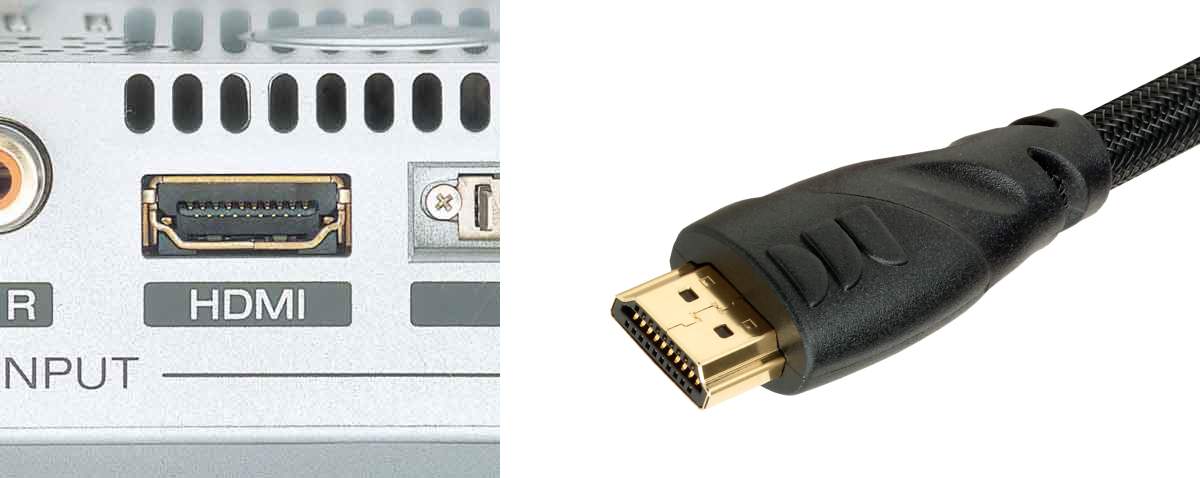
\includegraphics[width=0.60\textwidth]{graphics/hdmi.png}
		\caption{HDMI-kontakt (venstre) og kabel (h\o yre)}
		\label{fig:hdmi}
		\end{figure}
		
		Intensity er et HDMI capture card fra Blackmagic Design. Det er et stykke maskinvare som kan settes inn i en PC for \aa \space gj\o re det mulig \aa \space koble enheter til denne PC-en gjennom HDMI. Kortet kobles til PCI-express-porten i PC-en og har to HDMI-kontaktpunkter: inngang og utgang (se figur \ref{fig:intensity}).
		
		For \aa \space kunne f\aa \space ut bilde fra HD kameraet trengte vi HDMI input port som overf\o rer data i en s\aa \space stor hastighet slik at vi slipper \aa \space komprimere bildestr\o mmen. Vi valgte Blackmagic Intesity card som gir den beste og siste teknologien innen HDMI til Windows eller Mac OS. Intesity kortet har en HDMI inngang for HD kameraer som gir den h\o yeste kvalitet p\aa \space bilde. HDMI kan lese ukomprimert bildestr\o m direkte fra kameraet. Bildestr\o mmen er i 1080i (interlaced) det vil si at bilde har en oppl\o sning p\aa \space 1920�1080 piksler. 1080 linjer i vertikal retning og 1920 linjer i horisontal retning. Interlaced betyr at kameraet tar opp bilder med et alternerende sett med linjer slik at oddetallslinjene og partallslinjene oppdateres annenhver gang. Det vil si at det trengs to oppdateringer for \aa \space skape et fullstendig bilde, man \o ker bildekvaliteten av et videosignal uten \aa \space \o ke b\aa ndbredden. N\aa r bildet skal vises p\aa \space skjerm utf\o res det en deinterlacing som er en teknikk for \aa \space konvertere interlaced bildestr\o m til progressive bildestr\o m. Hvis det er 1080p (progressive) trenger bildestr\o mmen kun \aa \space oppdateres en gang for \aa \space f\aa \space et fullstendig bilde, at alle linjene vertikalt blir skannet ved en oppdatering. 
		 
		\begin{figure}[h]
		\centering
		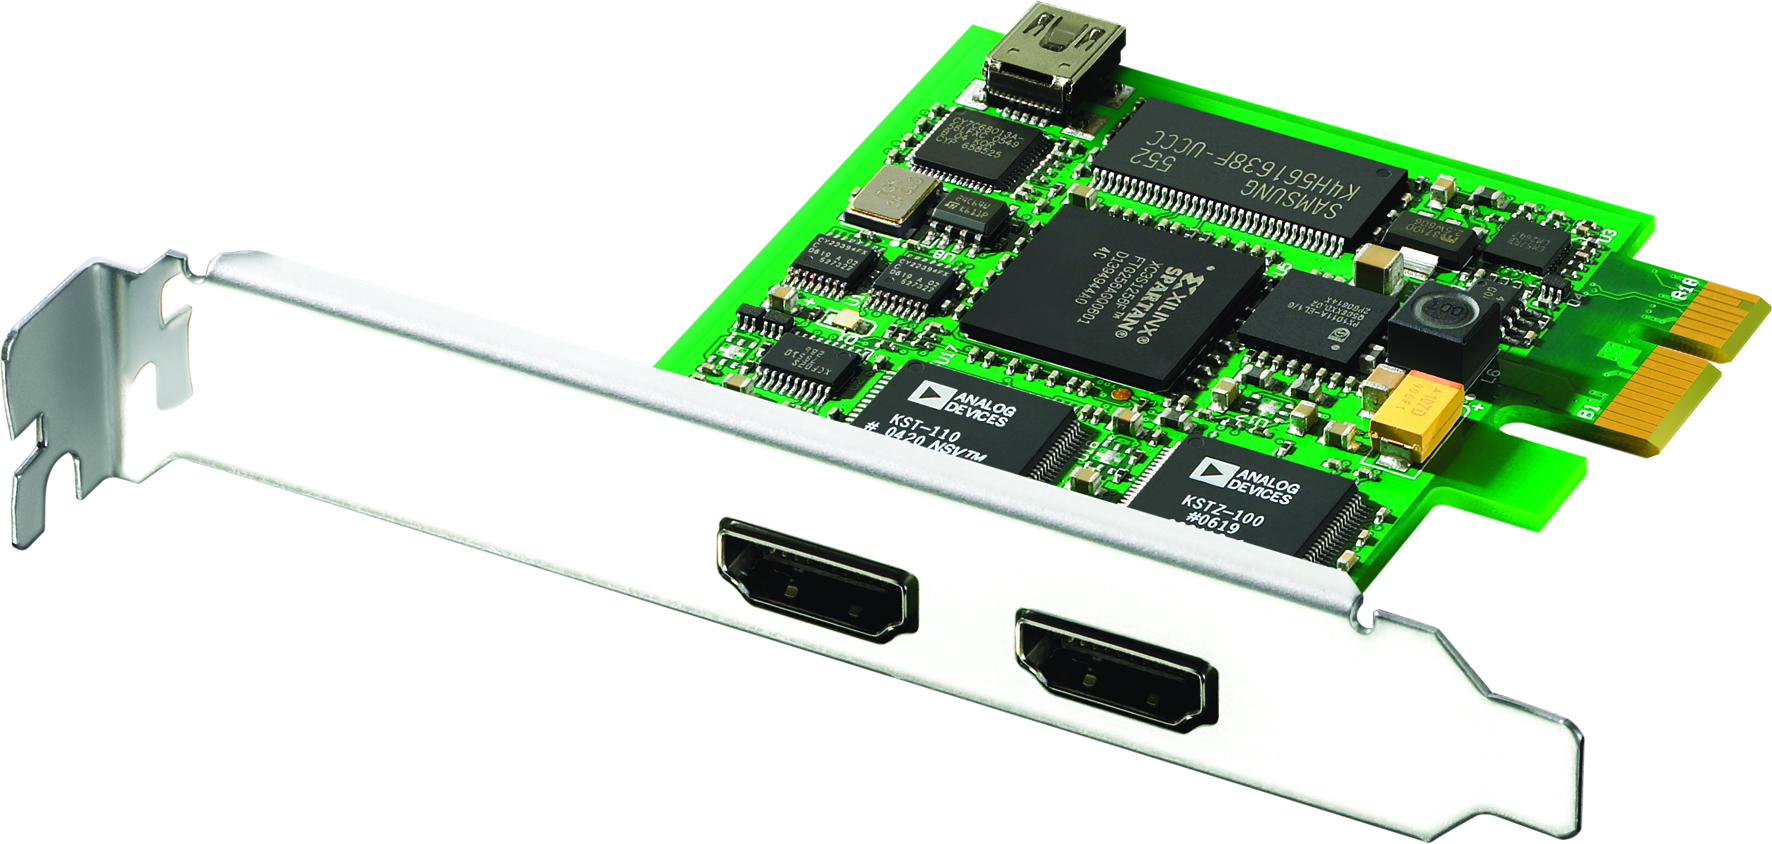
\includegraphics[width=0.60\textwidth]{graphics/intensity.png}
		\caption{Intensity fra Blackmagic Design}
		\label{fig:intensity}
		\end{figure}
	
	\subsection{DirectShow}
	
		DirectShow er et rammeverk og programvaregrensesnitt for \aa \space h\aa ndtere multimedia p\aa \space PC-er. Det er utviklet av Microsoft og gj\o r det mulig \aa \space spille av og ta opp media (typisk lyd og/eller bilde) gjennom et felles grensesnitt, og abstraherer bort maskinvaren. Bildene fra videokamera koblet til et Intensity-kort er tilgjengelig gjennom DirectShow. DirectShow er tilgjengelig gratis fra Microsofts nettsider.
		
	\subsection{Infrar\o dt lys}

		Infrar\o d lys er elekektromagnetisk str\aa ling av b\o lgelengder lengre enn b\o lgelengdene til synlig lys. Det synlige lyset har b\o lgelengder mindre enn 750nm. Ordet infra kommer fra latinsk og betyr under, og r\o d er den fargen innenfor det synlige spekteret som har den lengste b\o lgelengden. Det infrar\o de lyset som ligger n\ae rmest det synlige lys har mye av de samme egnskapene som det synlige lyset bortsett fra at det er usynlig for det mennesklige \o yet. Infrar\o dtlys er derfor mye brukt til blant annet overv\aa kning og nattkamera, i tillegg til ignaler i elektriske kontroller. Infrar\o d str\aa ling med lengre b\o lgelengder er mer knyttet til varmeproduksjon og varmesensitive kameraer som er mye brukt i romfartsindustri og v\aa penindustri.

		I dette prosjektet er det en fordel \aa \space bruke infrar\o dt lys fordi et lyspunkt som er synlig for det mennesklige \o yet kan v\ae re forstyrrende for brukeren og det kan blande seg med andre lyskilder i omgivelsene rundt som vil gj\o re det vanskligere finne punktene vi \o nsker under prosesseringsarbeidet. 

\section{\AA \space spore punkter i et bilde (Holger)}

	